% !TeX spellcheck = en_US
\documentclass{beamer}
\usetheme{Pittsburgh}
\usepackage{graphicx}
\usepackage{amsmath, amssymb}
\usefonttheme{serif}
\usepackage{siunitx}
\title{Interim progress report}
\author{Axel Fritz \& You Ming}
\date{\today}
\newcommand{\happy}{:)}
\newcommand{\sad}{:(}
\begin{document}
\begin{frame}[plain]
    \maketitle
\end{frame}
\section{Recap on Project}

	\begin{frame}{Project background}
		Physical models:
		\begin{itemize}
			\item Fluid dynamics (Navier-Stokes eqns.)
			\item Heat conduction (Heat eqn.)
		\end{itemize}

		
		
		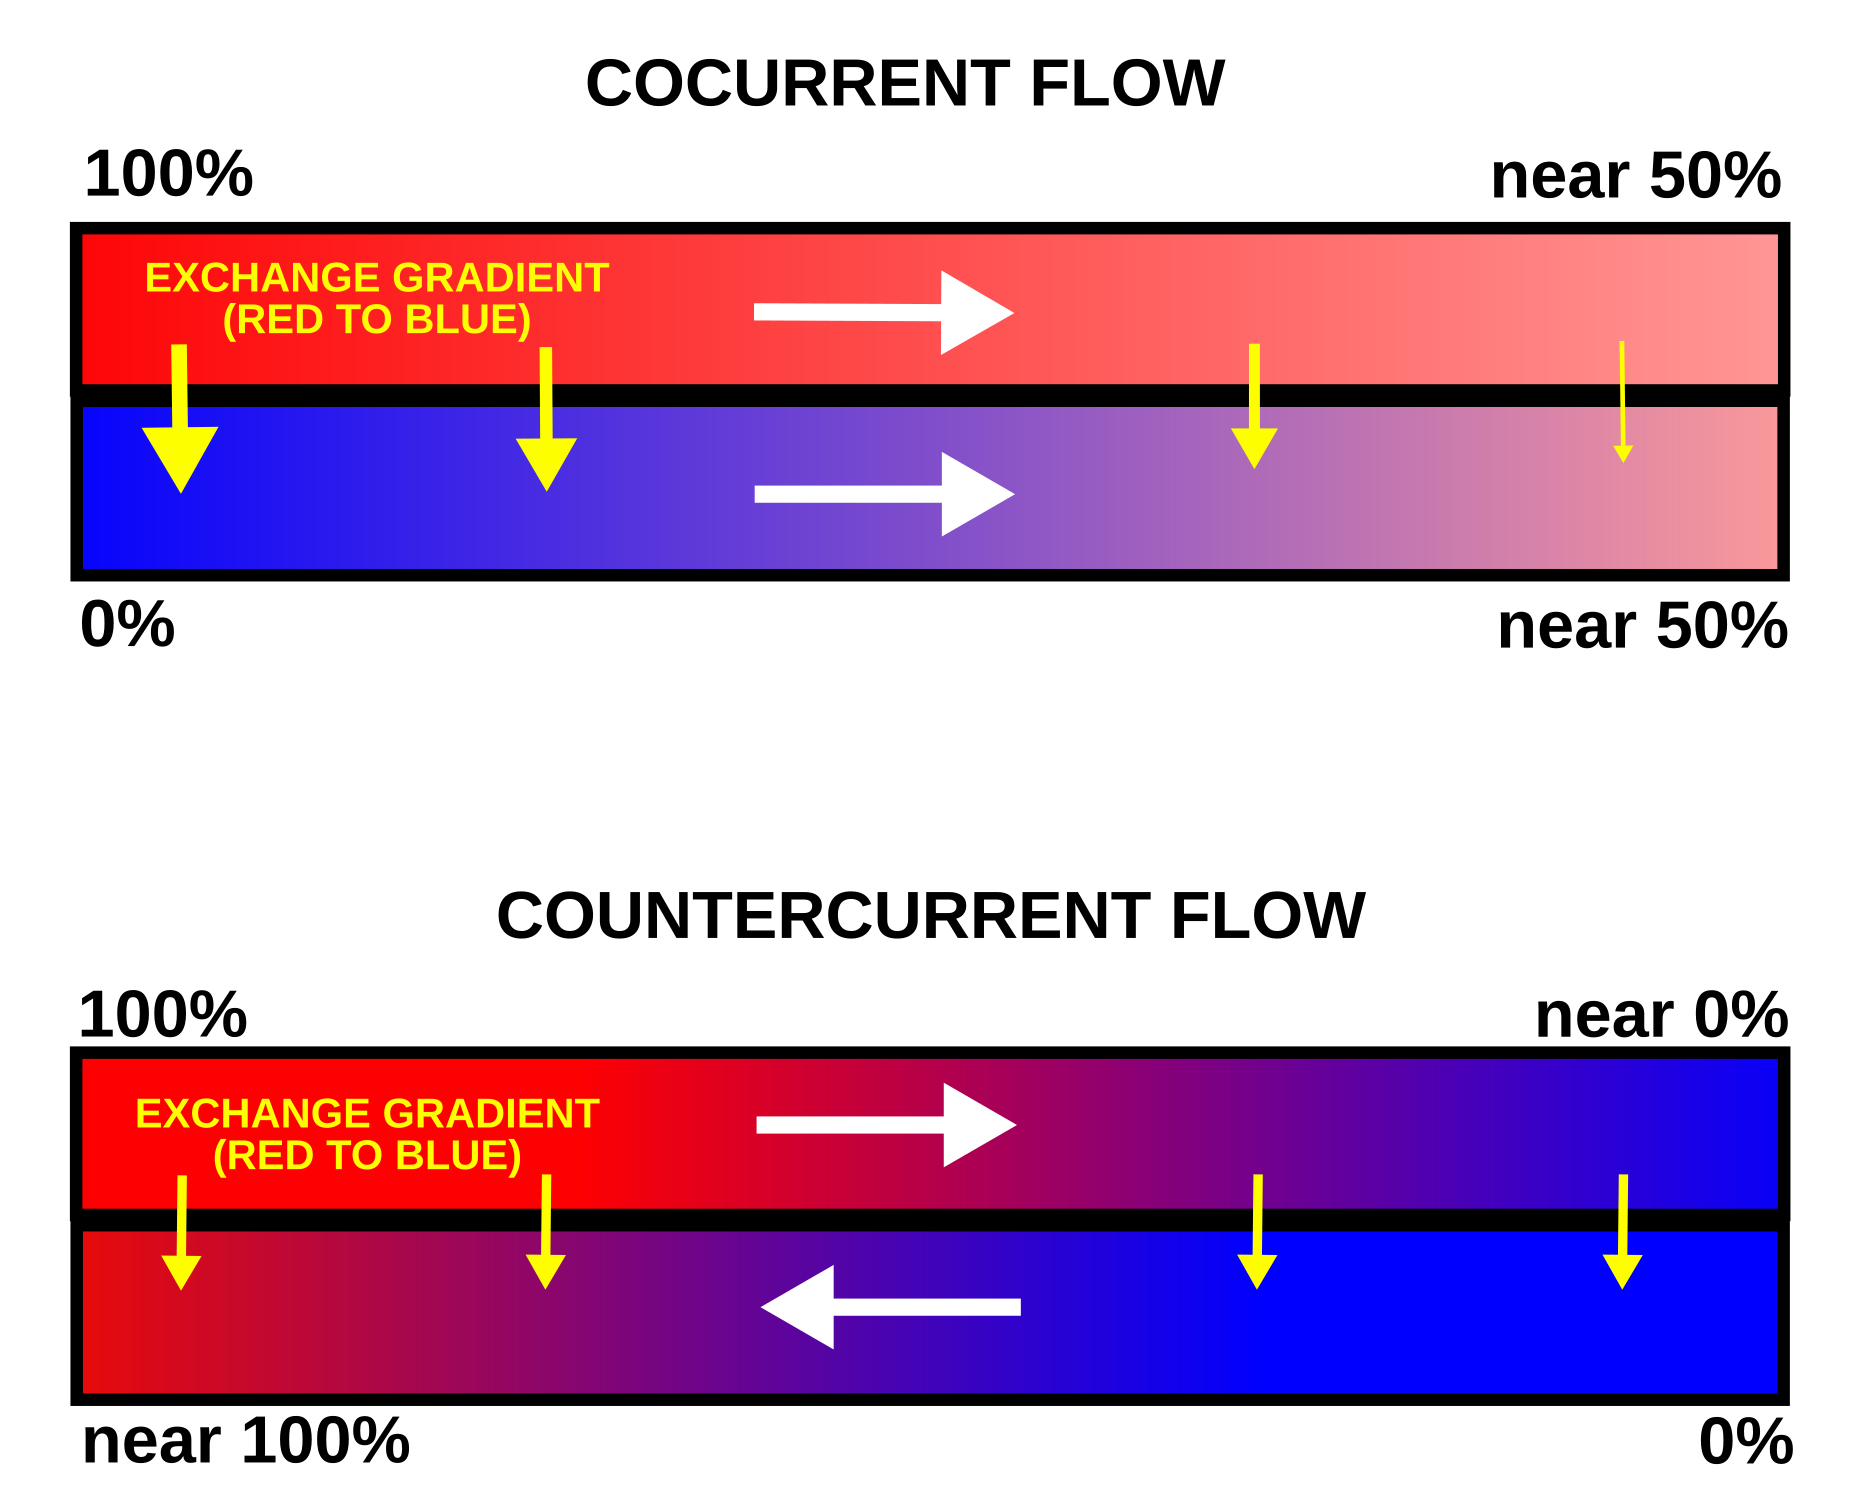
\includegraphics[width=0.45\textwidth]{imgs/heatdiagram.png}
	\end{frame}
	\begin{frame}{Project background}
		How is it justified to write an entire project about something so simple and well documented?
		\begin{itemize}
			\item Heat exchangers are traditionally evaluated by use of a body-fitted mesh
			\item For complex geometries, this is unfeasible
			\item Warrants the investigation into alternative methods (Brinkman's method)
			\item We are basing much of the theory on previous work from \emph{Dalian University} and \emph{University of Science and Technology of China}, paper titled \emph{Meshless Optimization of Triply Periodic Minimal Surface Based Two-Fluid Heat Exchanger} by Jiang~et~al. 
		\end{itemize}
	\end{frame}
\section{Progress}
	\begin{frame}{Fluid flow}
		Initially we implemented a simple model for fluid flow using the Brinkman method (left fig.), comparing it to the same geometry evaluated using traditional methods (right fig.). 
		
		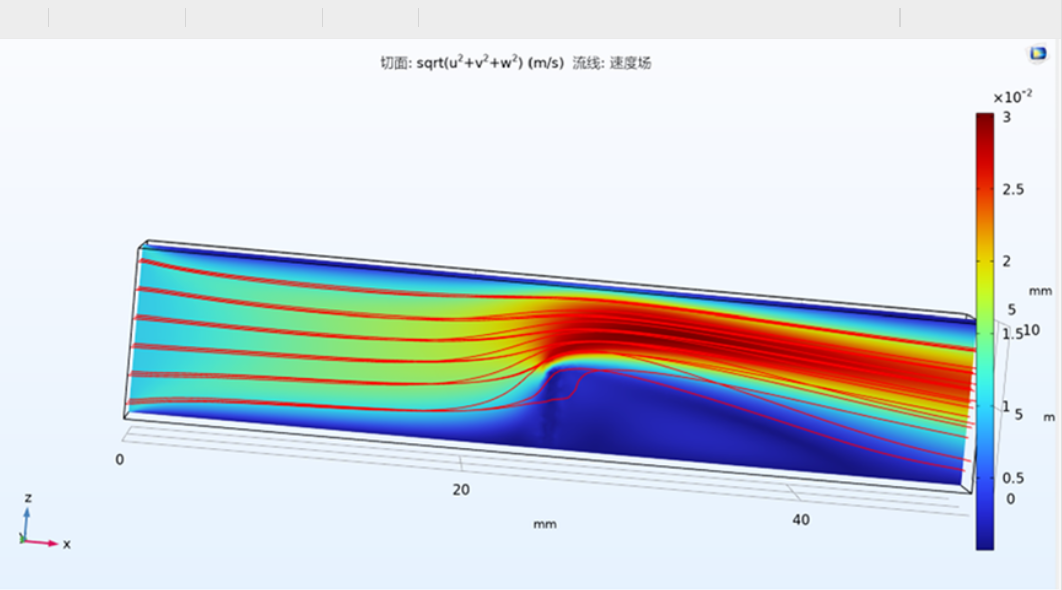
\includegraphics[width=0.45\textwidth]{imgs/youming1}
		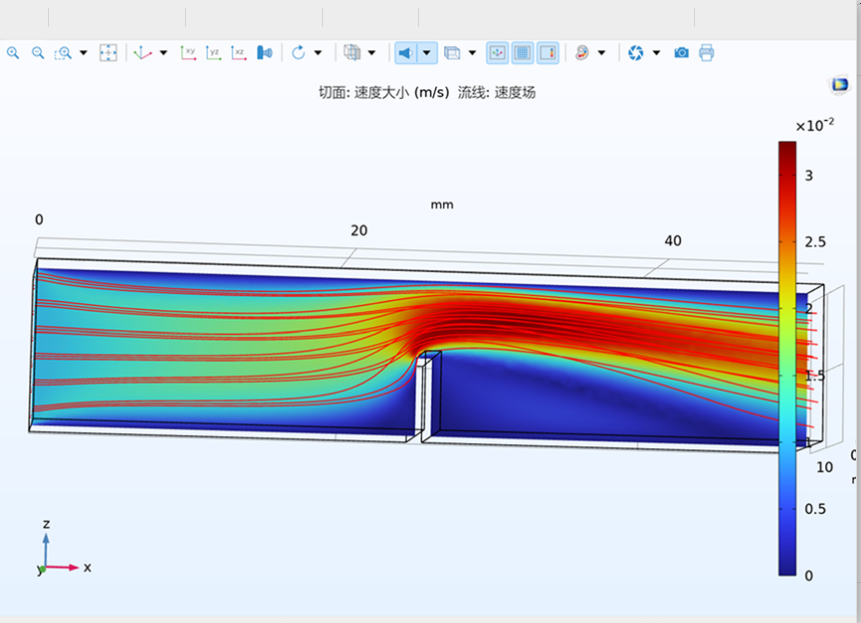
\includegraphics[width=0.45\textwidth]{imgs/youming2}
		
		\textbf{Note:} All figures in this presentation are slices from 3D models.  
		
	\end{frame}

	\begin{frame}{Channel separation}
		Critical to the performance of the model is that the two channels are adequately separated, i.e. that there is no flow between the two fluids. 
		
		Simply implementing the Brinkman method 'as-is' does not separate the channels enough. 
		
		\begin{center}
			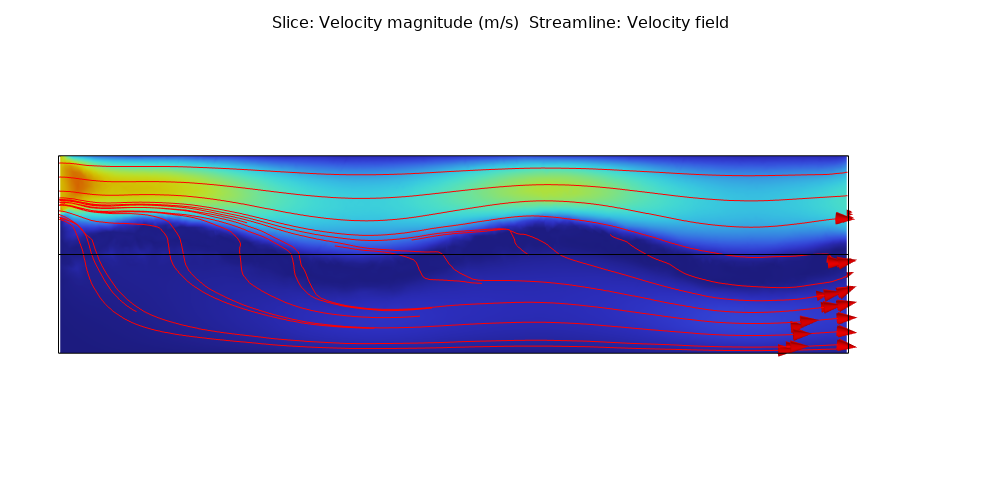
\includegraphics[width=0.45\textwidth]{imgs/separation_failed}
			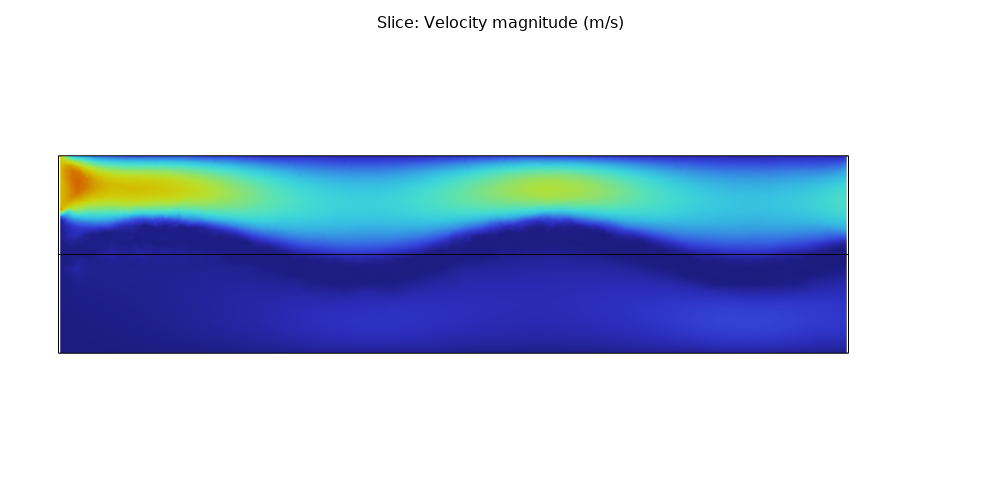
\includegraphics[width=0.45\textwidth]{imgs/separation_failed2.png}
			\sad
		\end{center}
		
		\begin{equation*}
			\text{Solid region: }|z-0.05-0.01\sin(10\pi x)|<0.005
		\end{equation*}
	\end{frame}
	
	\begin{frame}{Single channel}
		For a single channel we can define \emph{both} the wall and other channel so behave like solids, by changing the solid region to:
		\begin{equation*}
		z-0.05-0.01\sin(10\pi x)<0.005. 
		\end{equation*}
		This renders:
		
		\centering
		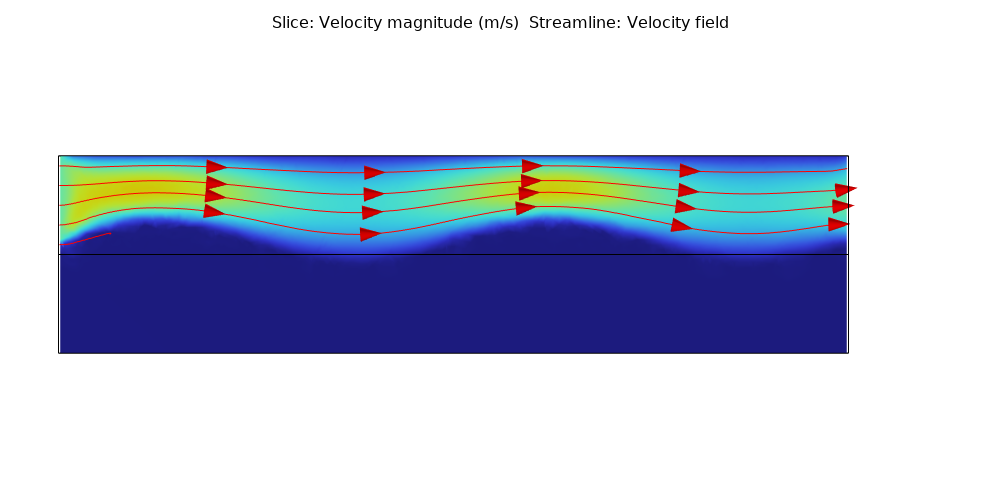
\includegraphics[width=0.9\textwidth]{imgs/sep_1ch_sl}
		\happy
	\end{frame}
	\begin{frame}{Dual channels}
		Luckily the Comsol framework can be nicely adjusted to incorporate two channels in the same model:
		
		\centering
		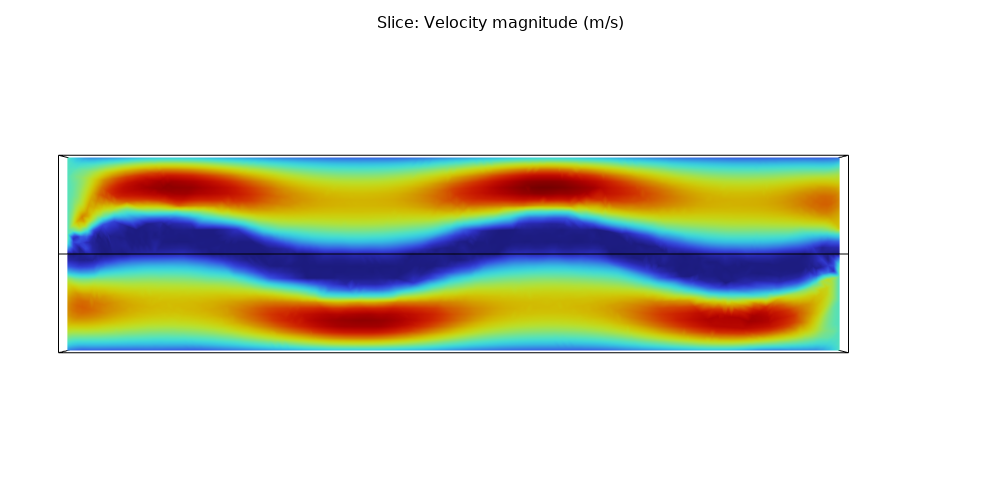
\includegraphics[width=0.49\textwidth]{imgs/sep_2ch}
		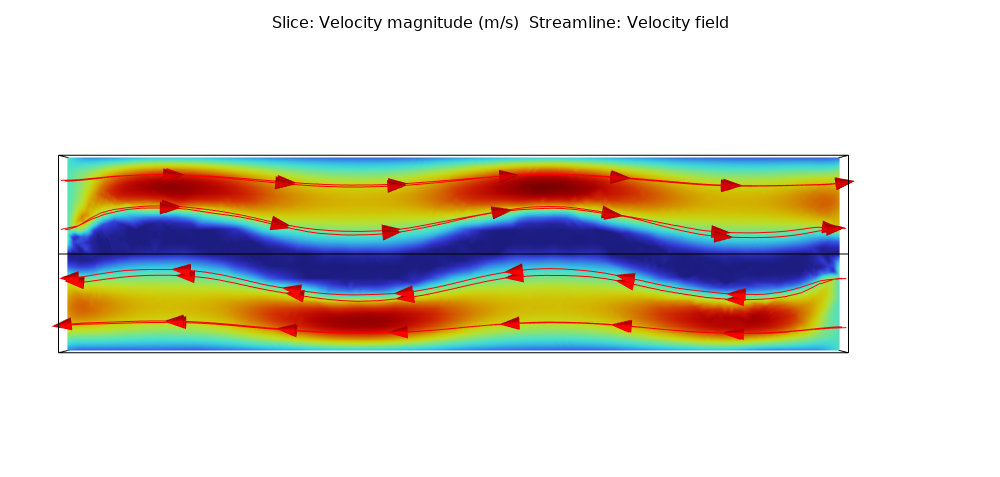
\includegraphics[width=0.49\textwidth]{imgs/sep_2ch_sl}
		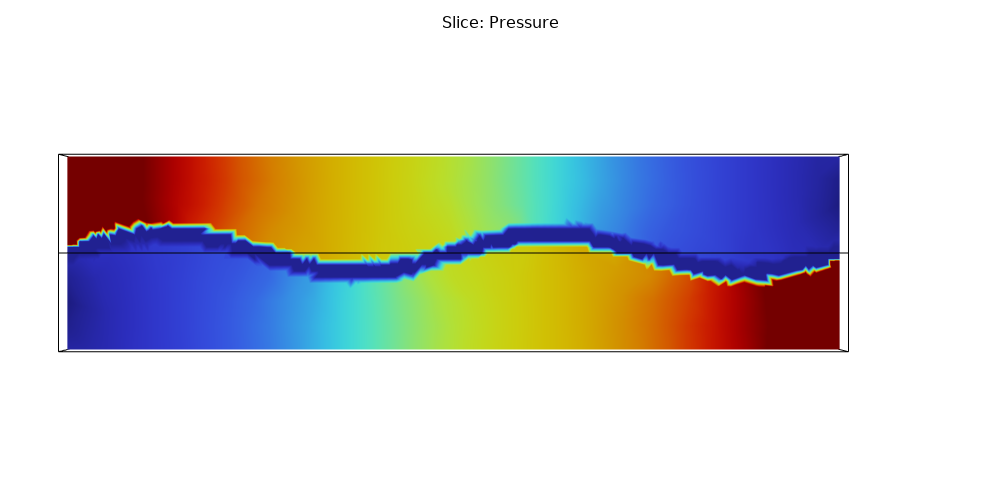
\includegraphics[width=0.49\textwidth]{imgs/sep_2ch_p}
		\begin{align*}
			z-0.05-0.01\sin(10\pi x)&<0.005 \tag{Upper channel} \\
			z-0.05-0.01\sin(10\pi x)&>-0.005 \tag{Lower channel}
		\end{align*}
		
	\end{frame}
	\begin{frame}{Heat transfer}
		Using the same model as before we can turn on the \emph{Heat Transfer in Fluids} module and solve for the temperature distribution. The thermal conductivity is set to \qty{0.6}{\W\per\m\per\K} for water and \qty{400}{\W\per\m\per\K} for copper. From this we can see that the current design of the heat exchanger is very poor:
		
		\centering
		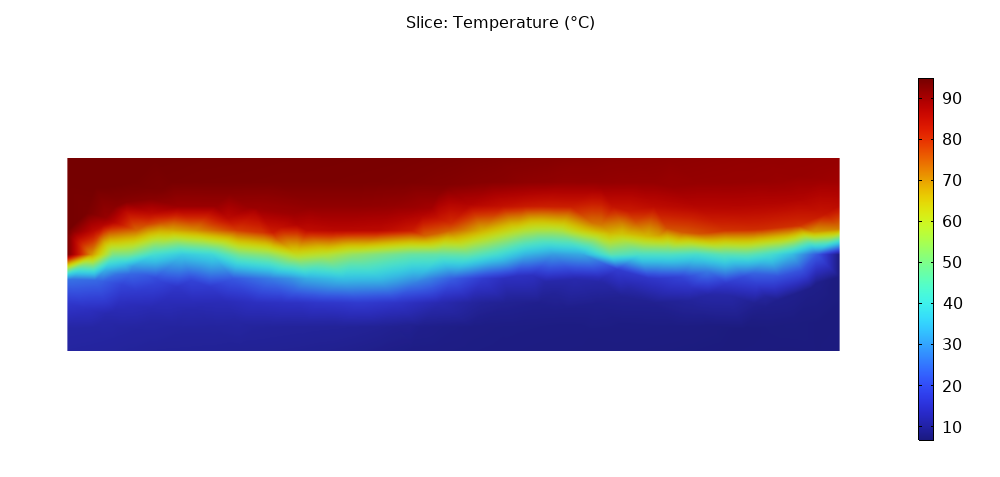
\includegraphics[width=0.7\textwidth]{imgs/sep_2ch_T}
	\end{frame}
\section{Future work}
	\begin{frame}{What is left to do}
		\begin{itemize}
			\item Begin investigating more complex geometries
			\item More thoroughly analysing the results and looking for numerical issues with the models. 
		\end{itemize}
	\end{frame}
\end{document}
